% PRELIMINARY RESULTS from the Python prototype (tgdiff/, 7 Nov. 2026). To be replaced by the SUMO campaign.
\subsection{Setup}
The prototype simulates a 1.5~km four-lane highway with three RSUs (coverage 300~m, MEC servers at 12~GHz), a cloud (60~GHz, 80~ms one-way backhaul) and vehicles at 18--32~m/s, about 30\% of them helpers with 4~GHz of spare capacity and a V2V range of 160~m (Table~\ref{tab:params}). Each vehicle generates tasks as a Bernoulli process; RSUs broadcast queue states every 250~ms, so all policies decide on stale reports. Unless stated otherwise, an episode lasts 60~s with 50 vehicles and 0.7 tasks per vehicle per second, and each result is the mean and standard deviation over three evaluation seeds.

Under attack, RSU-2 drops 60\% of its tasks (A1), a fraction $m$ of helpers drop 80\% of theirs (A2), and all malicious nodes report an empty queue (A3). The twin synchronisation error is $\sigma_{tw}=20$~ms and $\gamma=5$~s$^{-1}$.

\begin{table}[t]
\caption{Simulation parameters of the prototype}\label{tab:params}
\centering\footnotesize
\begin{tabular}{@{}ll@{}}
\toprule
Parameter & Value \\ \midrule
Road, lanes, vehicle speed & 1.5 km, 4, 18--32 m/s \\
RSUs, coverage, MEC capacity & 3, 300 m, 12 GHz \\
Vehicle / helper / cloud CPU & 1 / 4 / 60 GHz \\
V2I / V2V bandwidth & 20 / 10 MHz \\
V2V range & 160 m \\
SNR model & $\Gamma_0=30$ dB at $d_0=50$ m, $\alpha=3$ \\
Task size / workload & U(1,4) Mbit / U(0.3,1.5) Gcycles \\
Task deadline & U(0.4,1.0) s \\
Transmit power, $\kappa$, $\omega$ & 0.5 W, $10^{-27}$, 0.6 \\
Beacon, $\sigma_{tw}$, $\gamma$ & 250 ms, 20 ms, 5 s$^{-1}$ \\
Noise levels $T$, DDIM steps $K$, $\lambda$ & 20, 10, 1.0 \\
Denoiser & MLP 3$\times$256, Adam, 4000 it. \\
Training data & 65{,}099 decisions, 30 episodes \\
\bottomrule
\end{tabular}
\end{table}

\textbf{Baselines.} \emph{Greedy} picks the target with the lowest estimated cost from the reports. \emph{Greedy+Trust} does the same among targets with $\tau_j\ge0.5$. \emph{BC-MLP} is a behaviour-cloning classifier with the same inputs as \tgd{}, including trust and twin deviation. \emph{Diff} is a diffusion policy as in the literature, trained on the same data but without trust inputs or guidance. \emph{Expert} is the privileged expert used to generate the data, an upper bound that knows ground truth.

\subsection{No Attack}
Without attacks, all policies complete 99.0--100\% of the tasks on time for 20 to 80 vehicles. \tgd{} reaches 100\% with 60 and 80 vehicles, but its mean latency at 40 vehicles is 188~ms against 139~ms for Greedy+Trust: in this setting, the learned policies do not yet match the trust-aware heuristic on latency. \todo{réduire cet écart par l'affinage avec un critique Q}

\subsection{Malicious Nodes}
Fig.~\ref{fig:malicious} varies the share of malicious helpers, with the black-hole RSU and false reports active. Greedy loses about 29\% of its tasks as soon as attackers appear, because false reports attract it to malicious nodes. The unprotected diffusion policy completes only 85.3--88.5\% of the tasks: it cannot observe trust and follows the falsified states. \tgd{} keeps 99.9--100\%, close to the expert; Greedy+Trust (99.0--99.5\%) and BC-MLP (99.2--99.9\%) also resist, since both see the trust signal.

\begin{figure}[t]
\centering
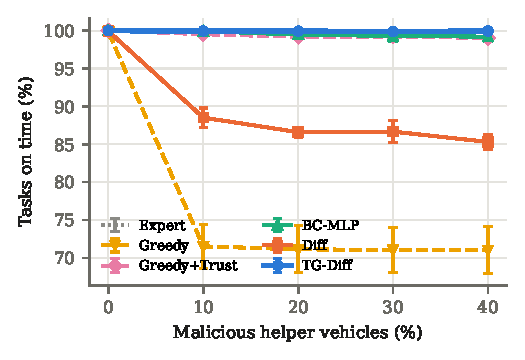
\includegraphics[width=\columnwidth]{figures/fig_malicious.pdf}
\caption{Tasks completed on time versus the share of malicious helper vehicles, with a black-hole RSU and false state reports (mean $\pm$ std, 3 seeds).}
\label{fig:malicious}
\end{figure}

\subsection{Data Poisoning}
Fig.~\ref{fig:poison} retrains the learned policies on data in which a fraction $\rho$ of the samples offering a malicious option are relabelled to it, and evaluates them with 30\% malicious helpers. Trust \emph{inputs} alone do not protect a learned policy against poisoning: BC-MLP falls from 99.3\% to 91.2\% as $\rho$ grows to 30\%. \tgd{} stays between 98.7\% and 99.7\%, because the guidance term suppresses untrusted targets at decision time whatever the denoiser learned.

\begin{figure}[t]
\centering
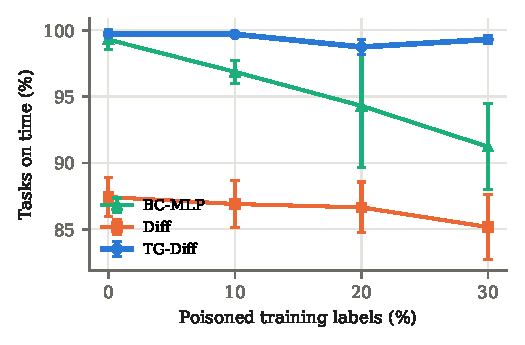
\includegraphics[width=\columnwidth]{figures/fig_poison.pdf}
\caption{Tasks completed on time versus the share of poisoned training labels, with 30\% malicious helpers (mean $\pm$ std, 3 seeds).}
\label{fig:poison}
\end{figure}

\subsection{Decision Time}
Fig.~\ref{fig:steps} varies the number of DDIM steps $K$. The measured decision time on a two-core CPU grows from 0.19~ms at $K=1$ to 2.34~ms at $K=20$, small compared with deadlines of 0.4--1~s. Success barely depends on $K$ in this discrete setting (99.2--99.9\% for \tgd{}), so few steps suffice; richer action spaces may need more.

\begin{figure}[t]
\centering
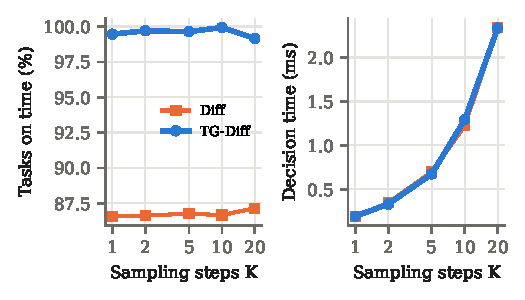
\includegraphics[width=\columnwidth]{figures/fig_steps.pdf}
\caption{Effect of the number of sampling steps $K$ on tasks completed on time (left) and on the measured decision time (right), with 30\% malicious helpers.}
\label{fig:steps}
\end{figure}

\subsection{Ablation and Value of the Digital Twin}
Table~\ref{tab:ablation} removes one component at a time with 30\% malicious helpers and 20\% poisoned labels. Trust guidance is the decisive component: without it, success falls from 99.0\% to 91.7\%. Removing the trust input costs 1.2 points and adds 33~ms of latency.

\begin{table}[t]
\caption{Ablation with 30\% malicious helpers and 20\% poisoned labels}\label{tab:ablation}
\centering\footnotesize
\begin{tabular}{@{}lccc@{}}
\toprule
Variant & On time (\%) & Latency (ms) & Lost tasks \\ \midrule
\tgd{} (full) & 99.0 $\pm$ 0.4 & 191 & 2 \\
without trust input & 97.8 $\pm$ 1.2 & 224 & 0 \\
without trust guidance & 91.7 $\pm$ 3.4 & 169 & 169 \\
without digital twin & 98.9 $\pm$ 0.5 & 211 & 0 \\
Diff (no trust) & 85.4 $\pm$ 2.2 & 180 & 300 \\
\bottomrule
\end{tabular}
\end{table}

In this setting the twin brings no gain in success, because malicious nodes also drop tasks and the beta reputation detects them. To isolate the twin, we ran a second scenario in which malicious nodes \emph{only} lie about their queues and never drop tasks, under heavy load (1 task per vehicle per second). Behaviour-based trust cannot see these nodes: Greedy+Trust without the twin completes 74.0\% (60 vehicles) and 78.0\% (80 vehicles) of the tasks, with mean latencies of 2.7~s and 3.5~s caused by congestion at the lying nodes. With the twin, the same heuristic reaches 100\% at 173 and 180~ms, and \tgd{} reaches 100\% at 172 and 170~ms against 198~ms without the twin.

\subsection{Discussion and Limitations}
Three findings stand out. First, an unprotected diffusion policy is markedly more vulnerable than a trust-aware heuristic, which confirms that generative decision makers are an attack surface. Second, trust must act \emph{inside} the generative process: trust features alone do not survive data poisoning, guidance does. Third, the twin is necessary against nodes that lie without dropping tasks. The prototype has limits that the full study will address: a synthetic highway instead of SUMO traces, a discrete action space in which a trust-aware heuristic is already strong, behaviour cloning instead of critic-based training, a single training seed, and attacks that do not adapt to the defense (e.g., nodes that build trust before attacking). \todo{campagne complète avec SUMO, 5 graines d'entraînement, attaquants adaptatifs}
